\documentclass[tikz]{standalone}
\usepackage{tikz}
\usetikzlibrary{calc, positioning}

\begin{document}
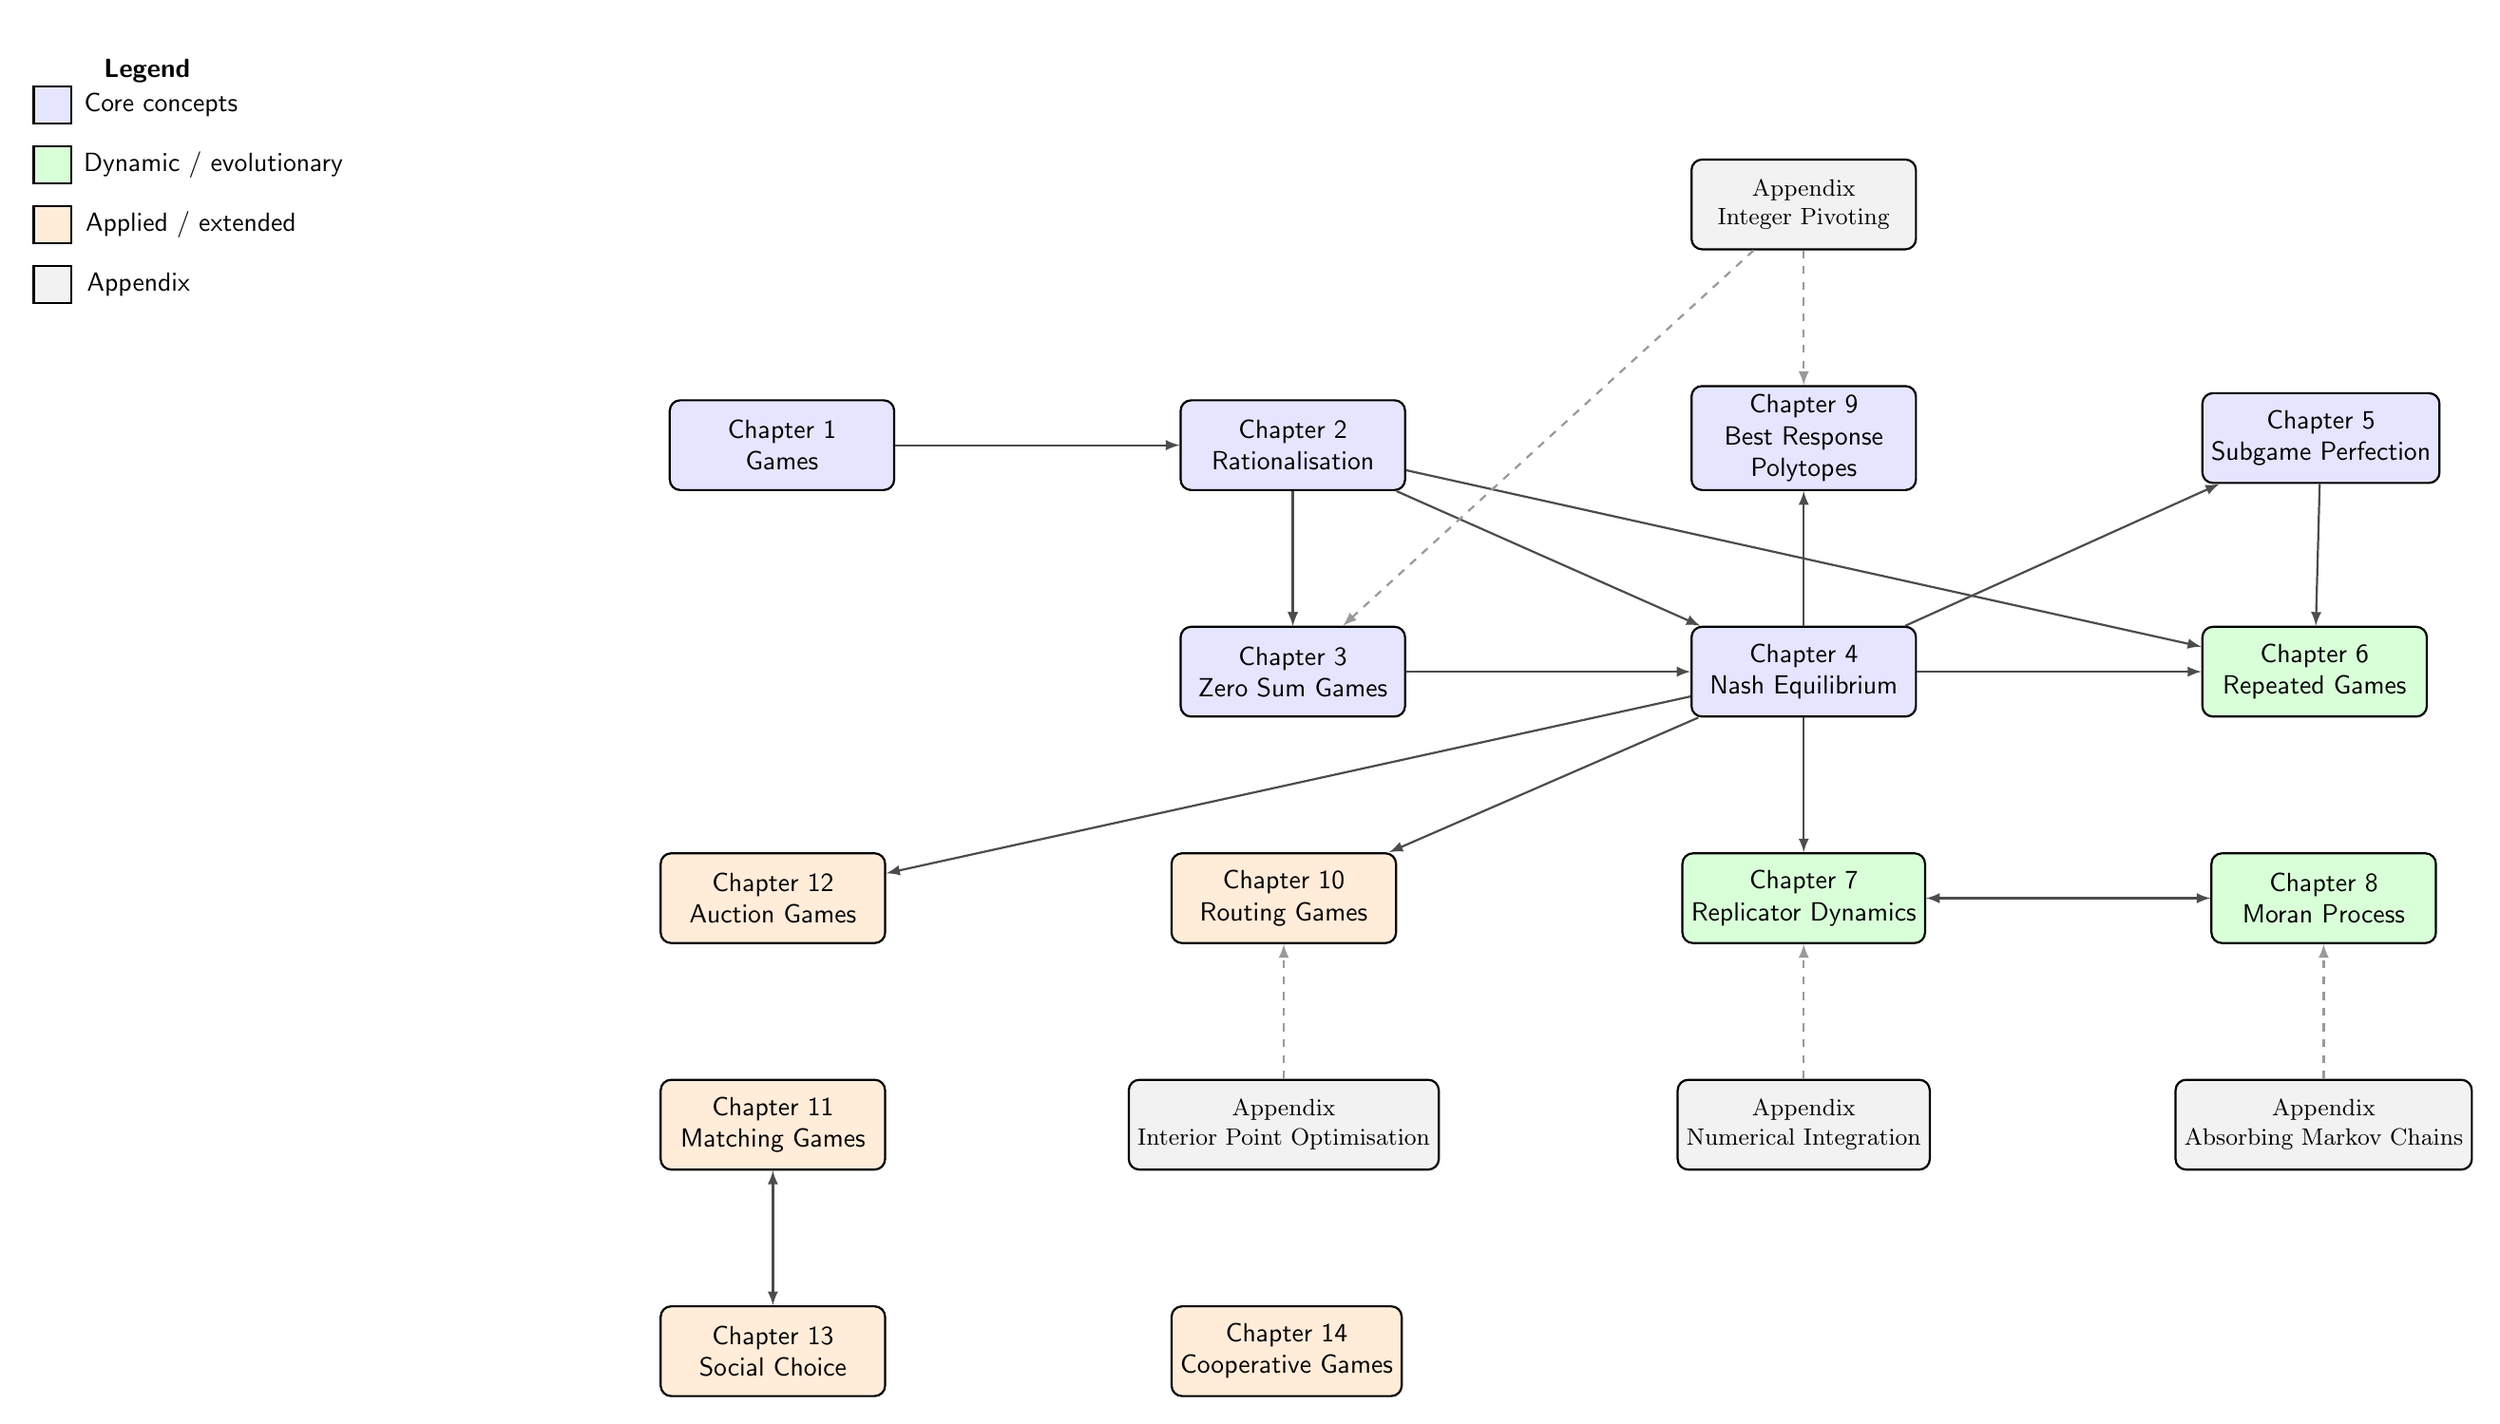
\begin{tikzpicture}[
    font=\sffamily,
    node distance=1.8cm and 3.8cm,
    every node/.style={
        draw,
        thick,
        rounded corners=4pt,
        minimum width=3cm,
        minimum height=1.2cm,
        align=center
    },
    base/.style={draw=black, fill=white},
    found/.style={base, fill=blue!10},
    dynamic/.style={base, fill=green!15},
    applied/.style={base, fill=orange!15},
    appendix/.style={base, fill=gray!10, font=\small},
    every path/.style={thick, draw=black!70, ->, >=latex},
    dashed path/.style={thick, draw=black!40, dashed, ->, >=latex}
]

% Legend in top-left corner
\node[anchor=west, draw=none] at (-10, 5) {\textbf{Legend}};
\draw[found] (-10, 4.3) rectangle ++(0.5, 0.5);
\node[ draw=none] at (-8.3, 4.55) {Core concepts};

\draw[dynamic] (-10, 3.5) rectangle ++(0.5, 0.5);
\node[ draw=none] at (-7.6, 3.75) {Dynamic / evolutionary};

\draw[applied] (-10, 2.7) rectangle ++(0.5, 0.5);
\node[ draw=none] at (-7.9, 2.95) {Applied / extended};

\draw[appendix] (-10, 1.9) rectangle ++(0.5, 0.5);
\node[ draw=none] at (-8.6, 2.15) {Appendix};

% Core game theory foundation
\node[found] (games) at (0, 0) {Chapter 1\\Games};
\node[found] (rationalisation) [right =of games] {Chapter 2\\Rationalisation};
\node[found] (zero_sum_games) [below =of rationalisation] {Chapter 3\\Zero Sum Games};
\node[found] (nash) [right=of zero_sum_games] {Chapter 4\\Nash Equilibrium};
\node[found] (brp) [above =of nash] {Chapter 9\\Best Response\\Polytopes};
\node[found] (subgame) [right=of brp] {Chapter 5\\Subgame Perfection};

% Dynamic and evolutionary games
\node[dynamic] (repeated) [right =of nash] {Chapter 6\\Repeated Games};
\node[dynamic] (replicator) [below=of nash] {Chapter 7\\Replicator Dynamics};
\node[dynamic] (moran)  [right=of replicator] {Chapter 8\\Moran Process};

% Extended equilibrium
\node[applied] (routing) [left=of replicator] {Chapter 10\\Routing Games};
\node[applied] (auction) [left=of routing] {Chapter 12\\Auction Games};

% Broader game models
\node[applied] (matching) [below=of auction] {Chapter 11\\Matching Games};

% Social and cooperative
\node[applied] (social_choice) [below =of matching] {Chapter 13\\Social Choice};
\node[applied] (coop) [right=of social_choice] {Chapter 14\\Cooperative Games};

% Appendices
\node[appendix] (numint) [below=of replicator] {Appendix\\Numerical Integration};
\node[appendix] (absorb) [below=of moran] {Appendix\\Absorbing Markov Chains};
\node[appendix] (ip) [below=of routing] {Appendix\\Interior Point Optimisation};
\node[appendix] (intpivot) [above=of brp] {Appendix\\Integer Pivoting};

% Edges
\draw (games) -- (rationalisation);
\draw (rationalisation) -- (zero_sum_games);
\draw (rationalisation) -- (nash);
\draw (rationalisation) -- (repeated);
\draw (rationalisation) -- (zero_sum_games);
\draw (zero_sum_games) -- (nash);
\draw (nash) -- (subgame);
\draw (nash) -- (repeated);
\draw (nash) -- (replicator);
\draw (nash) -- (brp);
\draw (nash) -- (routing);
\draw (nash) -- (auction);
\draw (subgame) -- (repeated);
\draw[<->] (moran) -- (replicator);
\draw[<->] (matching) -- (social_choice);

% Appendix edges
\draw[dashed path] (numint) -- (replicator);
\draw[dashed path] (absorb) -- (moran);
\draw[dashed path] (intpivot) -- (brp);
\draw[dashed path] (intpivot) -- (zero_sum_games);
\draw[dashed path] (ip) -- (routing);


\end{tikzpicture}
\end{document}
